% !TEX root = ../main.tex

We have implemented all aspects of our approach in $\mathtt{vigir\_behavior\_synthesis}$,\footnote{\scriptsize{\url{https://github.com/team-vigir/vigir_behavior_synthesis}}}
 a collection of Robot Operating System (ROS) Python packages.
Figure \ref{Fig:vigir_behavior_synthesis} depicts these packages as well as the nominal workflow.

\begin{figure}[t]
\centering
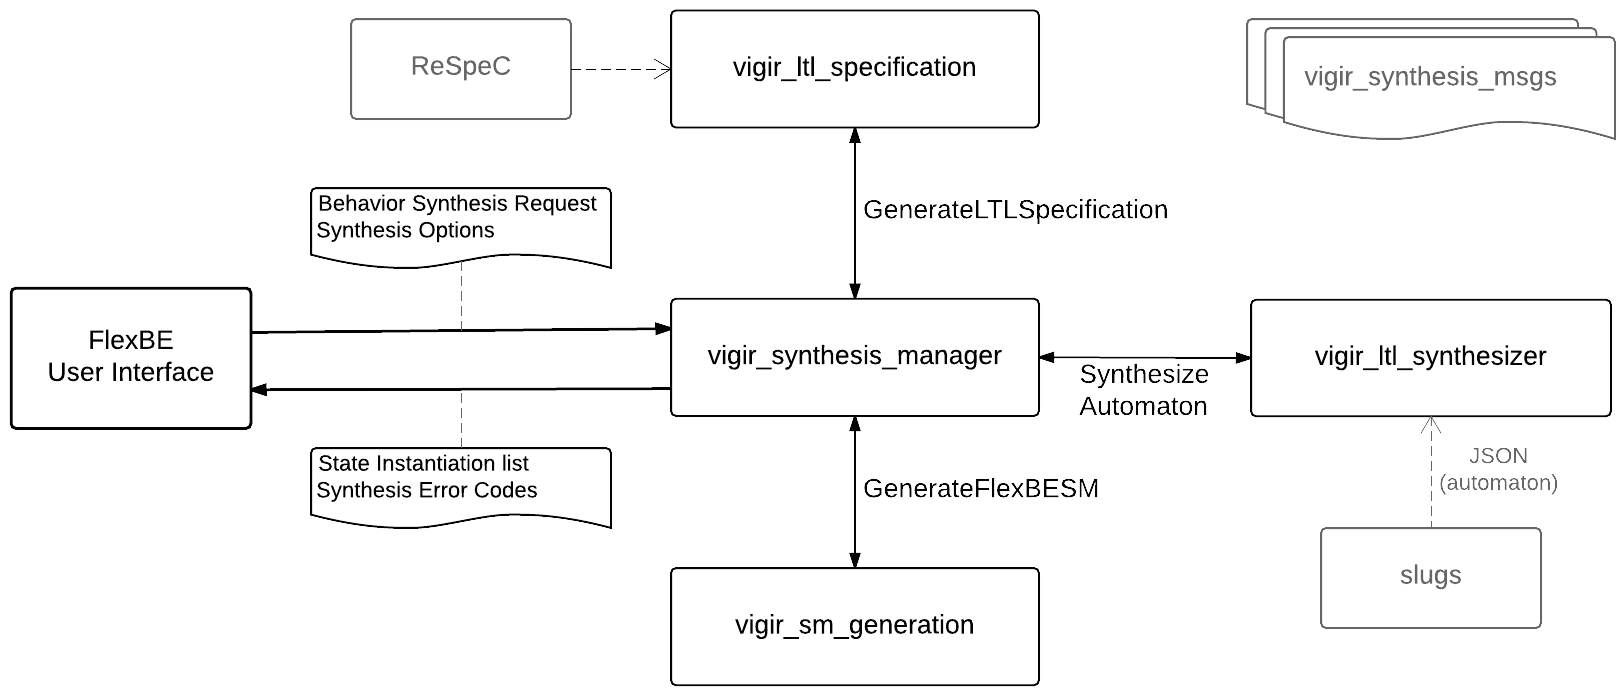
\includegraphics[width=0.99\columnwidth,clip]{./img/behavior_synthesis_packages.png}
\caption{Team ViGIR's ``Behavior Synthesis" ROS packages and the nominal workflow (clockwise, starting from the left).
\todo[inline, caption = {Update ROS packages figure}]{(i) Add ReSpeC to the image (move msgs to the left) (ii) Either number all arrows or none (iii) If I end up renaming LTLCompilation srv, update image accordingly.}
}
\label{Fig:vigir_behavior_synthesis}
\end{figure}

The synthesis action server ($\mathtt{vigir\_synthesis\_manager}$) receives a request from the user via FlexBE's GUI.
Given the user's input (initial conditions and goals), the server first requests a full set of LTL formulas for ATLAS from the LTL Compilation service ($\mathtt{vigir\_ltl\_specification}$).
The generation of the LTL formulas from Section \ref{S:ltl} is delegated to our ``Reactive Specification Construction kit," which is a ROS-independent Python framework\footnote{\scriptsize{\url{https://github.com/team-vigir/ReSpeC}}}.

\begin{figure}[t]
\centering
\fbox{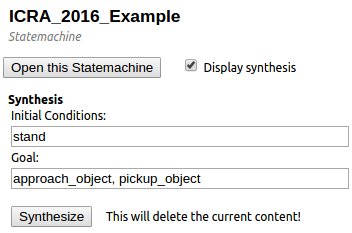
\includegraphics[width=0.90\columnwidth,clip]{./img/synthesis_menu_simple.png}}
\caption{Screenshot of the FlexBE Editor's synthesis menu.
}
\label{Fig:SynthesisMenuSimple}
\end{figure}

The LTL Synthesis service ($\mathtt{vigir\_ltl\_synthesizer}$) acts as a wrapper for an external synthesis tool (currently, \cite{SLUGS} is supported).
Upon request, it returns an automaton that is guaranteed to satisfy the LTL specification, if one exists.
Finally, the server requests a state instantiation message from the State Machine Generation service ($\mathtt{vigir\_sm\_generation}$).
The resulting message contains instructions that FlexBE can use to generate Python code: an executable state machine that instantiates the synthesized automaton.
The corresponding action, services, and messages are defined in the $\mathtt{vigir\_synthesis\_msgs}$ package.

% END